\documentclass[10pt]{beamer}

\usetheme[progressbar=frametitle]{metropolis}

\usepackage{booktabs}
\usepackage[scale=2]{ccicons}

\usepackage{pgfplots}
\usepgfplotslibrary{dateplot}

\usepackage{xspace}
\newcommand{\themename}{\textbf{\textsc{metropolis}}\xspace}

\title{Dynamic Scalable State Machine Replication}
%\subtitle{A modern beamer theme}
\date{\today}
\author{
  Long Hoang Le\\
  \texttt{long.hoang.le@usi.ch}\\
  \and
  Eduardo Bezerra\\
  \texttt{eduardo.bezerra@usi.ch}\\
  \and
  Fernando Pedone\\
  \texttt{fernando.pedone@usi.ch}}
  
\institute{University of Lugano, Switzerland}
%\titlegraphic{
\includegraphics[height=1.5cm]{figures/logo}}

\begin{document}

\maketitle

\begin{frame}{Outlines}
  \setbeamertemplate{section in toc}[sections numbered]
  \tableofcontents[hideallsubsections]
\end{frame}

\section{Motivation}

\begin{frame}[fragile]{State Machine Replication}

  \begin{figure}
    % \includegraphics<1>[width=.8\textwidth]{figures/smr-1}
    % \includegraphics<2>[width=.8\textwidth]{figures/smr-2}
    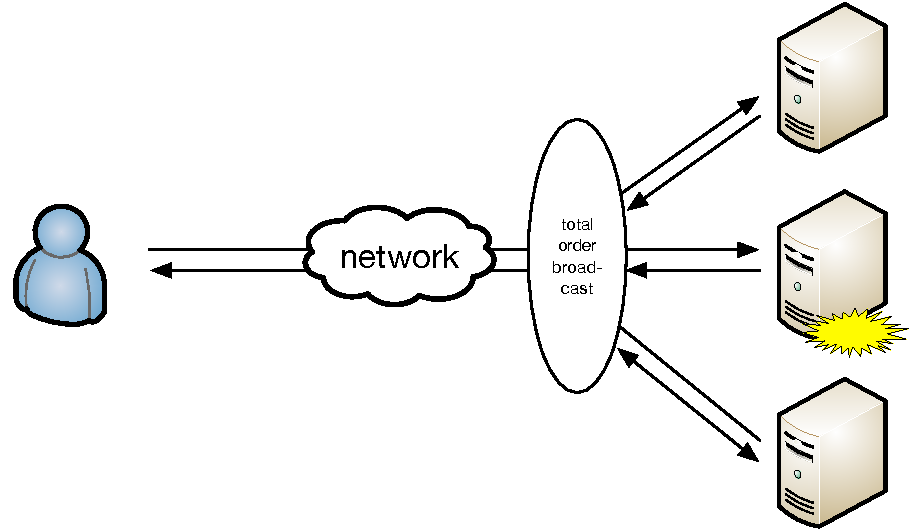
\includegraphics[width=.8\textwidth]{figures/smr-3}
  \end{figure}
\end{frame}

\begin{frame}[fragile]{State Machine Replication}

  Providing fault-tolerance, strong consistency
  \begin{itemize}
    \item All replicas start in the same initial state
    \item Apply same set of commands in the same order 
    \item The executions of commands are deterministic
    \item Proceed through the same set of states
  \end{itemize}
\end{frame}

\begin{frame}[fragile]{State Machine Replication}
  Production systems
  % Many production systems use this approach to tolerate crash faults:
    \begin{itemize}
      \item Google Spanner, Windows azure storage, CockroachDB, HydraBase, Chubby
    \end{itemize}
\end{frame}

\begin{frame}[fragile]{Scaling State Machine Replication}

  SMR lacks of scalability:
  \begin{itemize}
    \item Every replica executes all commands.
    \item Adding servers does not increase the maximum throughput
  \end{itemize}
  
  Different techniques have been developed to deal with these limitations
  \begin{itemize}
    \item Scaling up
    \item Scaling out
  \end{itemize}

\end{frame}

\begin{frame}[fragile]{Scalable State Machine Replication}

  Applies state partitioning
  \begin{itemize}
    \item Partitions application's state and replicates each partition
    \item Relies on an atomic multicast primitive %to consistently order commands within and across partitions
  \end{itemize}

  Guarantees strong consistency (i.e., linearizability)
  \begin{itemize}
    \item Provides execution atomicity
  \end{itemize}

  
\end{frame}

\begin{frame}[fragile]{Scalable State Machine Replication}
  Assumes a static workload partitioning
  \begin{itemize}
    \item Relies on static mapping
    \item Mapping does not need to be minimal
  \end{itemize}
  Expensive cost of multi-partition commands
  \begin{itemize}
    \item Partitions need to exchange signals
    \item Performance decreases when number of involved partitions increases
  \end{itemize}
  
\end{frame}

\section{Dynamic Scalable State Machine Replication}

\begin{frame}{System Model}
  Communication by message passing
  \begin{itemize}
    \item One-to-one communication use reliable multicast
    \item One-to-many communication relies on atomic multicast
    \item Messages can be lost, reordered, but not corrupted
  \end{itemize}
  Crash-stop failure model
  \begin{itemize}
    \item No Byzantine behavior
  \end{itemize}
  System is partially synchronous
  \begin{itemize}
    \item No delay bound
  \end{itemize}
\end{frame}

\begin{frame}{General idea}
  \alert {Dynamically changing the partitioning}
  \begin{itemize}
    \item DS-SMR was designed to exploit workload locality
    \item Involved variables are moved to a single partition
    \item Command is executed against this partition
    \item Variable mapping managed by an Oracle partition
  \end{itemize}

  It distinguishes five types of commands
  \begin{itemize}
    \item $access(w), create(v), delete(v), move(v, Ps, Pd), consult(C)$
  \end{itemize} 

  Clients consult the oracle to know each variable's location

  Clients $retry$ if variables change location

  Clients fall back to S-SMR after a number of retries

\end{frame}

\begin{frame}{General idea}
  \begin{figure}
    \includegraphics<1>[width=1\textwidth]{figures/dssmr-1-1}
    \includegraphics<2>[width=1\textwidth]{figures/dssmr-1-2}
    \includegraphics<3>[width=1\textwidth]{figures/dssmr-1-3}
    \includegraphics<4>[width=1\textwidth]{figures/dssmr-2-0}
    \includegraphics<5>[width=1\textwidth]{figures/dssmr-2-1}
    \includegraphics<6>[width=1\textwidth]{figures/dssmr-2-2}
    \includegraphics<7>[width=1\textwidth]{figures/dssmr-2-3}
    \includegraphics<8>[width=1\textwidth]{figures/dssmr-2-4}
    \includegraphics<9>[width=1\textwidth]{figures/dssmr-2-5}
  \end{figure}
\end{frame}

\begin{frame}{Architecture}

  \includegraphics<1>[width=1\textwidth]{figures/arch-1}
  \includegraphics<2>[width=1\textwidth]{figures/arch-2}
  \includegraphics<3>[width=1\textwidth]{figures/arch-3}
  \includegraphics<4>[width=1\textwidth]{figures/arch-0}

  \only<1> {
    \begin{block}{Client}
      \begin{itemize}
        \item Application Client
        \item DS-SMR Client Proxy
      \end{itemize}
    \end{block}
  }
  \only<2>  {
    \begin{block}{Oracle}
      \begin{itemize}
        \item Application Oracle
        \item DS-SMR Oracle Proxy 
      \end{itemize}
    \end{block}
  }
  \only<3>  {
    \begin{block}{Server}
      \begin{itemize}
        \item Application Server
        \item DS-SMR Server Proxy 
      \end{itemize}
    \end{block}
  }
  \only<4>  {
    \begin{itemize}
      \item Clients atomically multicast commands to oracle and partitions
      \item Oracle and partitions exchange messages through reliable multicast
    \end{itemize}  
  }

  

\end{frame}

\begin{frame}{Performance optimizations}
  \begin{itemize}
    \item Caching
      \begin{itemize}
        \item Each client proxy has a local cache
        \item Client consults local cache to determine variable's location
        \item When retrying command, clients update cache
      \end{itemize}
    \item Under the assumption of locality, most consult queries will be accurately resolved by the client's cache
  \end{itemize}
\end{frame}

\begin{frame}{Performance optimizations}
  \begin{figure}
    \includegraphics<1>[width=1\textwidth]{figures/cache-retry}
  \end{figure}
\end{frame}

\section{Implementation}

\begin{frame}{Eyrie}
  %One of the main goals of Eyrie is to make the implementation of services based on Scalable SMR as easy as possible.
  Eyrie simplifies implementing services based on DS-SMR 

  Provides proxy layers 

  Allows application designers to override default behaviors

  \begin{itemize}
    \item The PRObject class
    \item The StateMachine class
    \item The OracleStateMachine class
  \end{itemize}
\end{frame}

\begin{frame}{Chirper}
  Social network application similar to Twitter

  State partitioning is based on users' interest

  Supports commands: 
  \begin{itemize}
    \item post
    \item getTimeline
    \item follow, unfollow
  \end{itemize}

\end{frame}


\section{Performance Evaluation}

\begin{frame}{Environment setup and configuration parameters}
  Running \emph{Chirper} under different loads and partitionings

  Partitioning: 2 replicas and 3 acceptors for each partition

  Number of partitions: 2, 4, and 8

  Workloads:
  \begin{itemize}
    \item Timeline
    \item Post
    \item Follow, Unfollow
    \item Mix
  \end{itemize}
\end{frame}

\begin{frame}{Results}
  \begin{figure}
    \includegraphics<1>[width=0.7\textwidth]{figures/experiment}
  \end{figure}
\end{frame}

\section{Conclusion}

\begin{frame}{Summary}
  \begin{itemize}
    \item S-SMR does not adapt to changing locality
    \item D-SSMR introduces dynamic repartitioning to S-SMR
    \item Results show that D-SSMR outperforms S-SMR when there is access locality
    \item Eyrie makes developing services based on DS-SMR much simpler
  \end{itemize}
  
\end{frame}

\plain{Questions?}

\end{document}
